\section{问题介绍}

\subsection{基于跨域表示学习的工业控制系统异常检测}

工业控制系统广泛应用于电力、制造、水利等关键基础设施,其安全性和稳定性至关重要。
一旦ICS受到攻击,可能会造成严重的损坏。
因此,针对ICS异常检测是十分重要的。
传统异常检测方法主要关注单一域中的指标,如网络域中的网络流量或物理域中的传感器数据,但ICS中不同域(如传感器的物理状态、网络通信流量等)的行为存在强相关性,仅分析单一域难以全面识别异常。
例如,网络攻击可能导致传感器数据异常,但某些攻击仅影响物理设备而不改变网络流量。
现有的方法如基于RNN\cite{mandic2001recurrent}、GAN\cite{creswell2018generative}或基于单域图的神经网络模型无法有效建模跨域关联,导致检测精度不足和误报率高。
文章\cite{zhan2024anomaly}在GDN\cite{deng2021graph}的基础上提出了一种基于跨域表示学习的ICS异常检测方法(MGDN),该方法能够学习多域行为的联合特征,并在不同的域内进行异常检测。
在构建跨域图来表示ICS中多个领域的行为之后,该方法可以利用图神经网络学习它们的联合特征。
由于异常在不同领域表现不同,利用多任务学习方法分别识别不同领域的异常并进行联合训练。

\subsection{基于异构图的大规模微服务系统性能问题诊断}

大规模微服务系统在运行过程中通常会产生大量的服务调用,尤其是在短时间内。
这意味着当检测到性能问题时,系统周围可能会有大量的调用记录。
这种海量的数据使得分析所有调用记录变得既低效又困难,而且根因定位的精度也会受到影响。
主要原因在于,其中许多服务调用与性能问题并无直接关系。
因此需要识别与性能问题有关的微服务调用。

大多数传统的方法识别异常的调用端口(即端口级),文章\cite{tao2024diagnosing}提出了一种基于服务级的异常检测方法(MicorDig)。
为了更准确地定位异常微服务,文章首先选择构建端口级调用图,然后,通过在图上执行广度优先搜索(Breadth-First Search,BFS)和异常检测来保留相关调用和相应的微服务。
如\cref{img:Port-level call graph}所示,圆圈表示端口级节点,同一个虚线椭圆内的端口属于同一个微服务,橙色的端口级节点为问题无关节点,虚线表示的调用为非异常调用。
最后,如\cref{img:Service-level call graph}所示,将图中的端口级节点聚合到服务级。

\begin{figure}[ht]
    \centering
    \begin{subfigure}{0.32\linewidth}
        \centering
        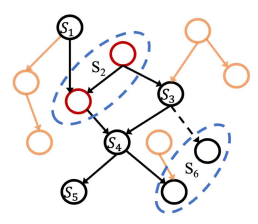
\includegraphics[scale = 0.6]{img/port-level call graph.png}
        \caption{端口级调用图}
        \label{img:Port-level call graph}
    \end{subfigure}
    \begin{subfigure}{0.32\linewidth}
        \centering
        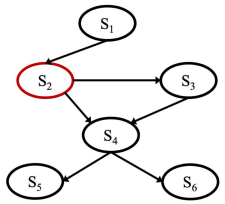
\includegraphics[scale = 0.6]{img/Service-level call graph.png}
        \caption{服务级调用图}
        \label{img:Service-level call graph}
    \end{subfigure}
    \begin{subfigure}{0.32\linewidth}
        \centering
        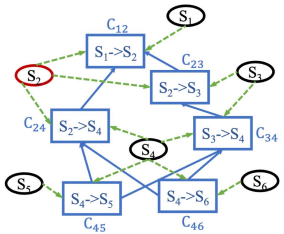
\includegraphics[scale = 0.55]{img/Service-level Heterogeneous Propagation Graph.png}
        \caption{服务级异构传播图}
        \label{img:Service-level Heterogeneous Propagation Graph}
    \end{subfigure}
    \caption{异构传播图的构造过程}
\end{figure}
